\PassOptionsToPackage{utf8}{inputenc}
\documentclass{bioinfo}
\copyrightyear{2020} \pubyear{2020}

\usepackage[colorlinks=true,urlcolor=black,citecolor=blue]{hyperref}
\usepackage[ruled,vlined]{algorithm2e}
\usepackage{multicol}

\access{Advance Access Publication Date: Day Month Year}
\appnotes{Manuscript Category}

\newcommand\st{\textbf{Stitcher}}
\newcommand\ix{\textbf{InXight Drugs}}
\newcommand\bangedup{\framebox{\parbox{\textwidth}{\it Dear Reviewer: Due to technical difficulties with our typesetting software, we were unable to generate proper references for this paper before the submission deadline. However, the complete ``source code'' and bibliographies of the paper are available at \url{https://github.com/ncats/stitcher/paper} should you have any concerns.}}}

\begin{document}
\firstpage{1}

\subtitle{Database and ontologies}

\title[Stitcher: An entity resolution framework]{Stitcher: An entity resolution framework for comprehensive data integration of approved drugs}
\author[Nguyen \textit{et~al}.]{Dac-Trung Nguyen,$^{\text{\sfb 1}}$
Ivan Grishagin,$^{\text{\sfb 1}}$
Daniel Katzel,$^{\text{\sfb 1}}$
Tyler Peryea,$^{\text{\sfb 1,2}}$ and Noel Southall\,$^{\text{\sfb 1},\ast}$}
\address{$^{\text{\sf 1}}$Division of Pre-clinical Innovation, National Center for Advancing Translational Sciences (NCATS), National Institutes of Health, USA\\
$^{\text{\sf 2}}$Present address: Office of Health Informatics, Office of Chief Scientist, Food and Drug Administration, USA}

\corresp{$^\ast$To whom correspondence should be addressed.}

\history{Received on XXXXX; revised on XXXXX; accepted on XXXXX}

\editor{Associate Editor: XXXXXXX}

\abstract{\textbf{Motivation:}
\\
\textbf{Results:} Text  Text Text Text Text Text Text Text Text Text  Text Text Text Text Text
Text Text Text Text Text Text Text Text Text Text Text Text Text  Text Text Text Text Text Text\\
\textbf{Availability:} The complete source code along with data and build instructions for \st{} is readily available on Github \url{https://github.com/ncats/stitcher}. The \ix{} resource is accessible at \url{https://drugs.ncats.io}.\\
\textbf{Contact:} \href{mailto:southalln@mail.nih.gov}{southalln@mail.nih.gov}\\
\textbf{Supplementary information:} Supplementary data are available at \textit{Bioinformatics}
online.\\%[2em]
%\bangedup
}

\maketitle

\section{Introduction}
As the volume of biological data continues to grow at an unprecedented rate, data de-duplication---also commonly known as record linkage or \emph{entity resolution}---is proportionally playing a prominent role in data integration. From the construction of training data for machine learning to building knowledge graphs as epistemological frameworks for artificial intelligence, proper entity resolution is essential in generating ground-truth data. The core challenge of entity resolution is in establishing \emph{uniqueness}. For well-defined entity types (e.g., gene, tissue, cell line), uniqueness is determined solely based on established identifiers and nomenclature; for other entity types (e.g., drug, disease, phenotype), however, uniqueness is not as well-established due to conceptual ambiguities in how entities are defined and represented. Take the disease entity type as an example. The discrepancy between the theoretical concept of ``disease entity'' from its clinical nosology \citep{Hucklenbroich14} is what makes disease entity resolution extremely challenging.

Herein we report on our recent data integration effort to build a comprehensive resource of drugs that have either been marketed or approved in the United States for human use. Such a resource is not only instrumental for drug repurposing but also serves as a valuable tool to further our understanding of the mechanistic properties of molecular targets \citep{Huang2019}. To the best of our knowledge, \ix{} is currently the most comprehensive resource of its kind. In the remainder of this paper, we discuss data integration challenges associated with drug data, conceptually as well as technically. This discussion serves as the backdrop for the development of \st, an entity resolution framework that we have developed to address the shortcomings of traditional approaches.

\subsection{What is a ``drug''?}
While the word is included within the name of the organization, the U.S. Food and Drug Administration (FDA) does not have a straightforward definition of the word ``drug.'' The Federal Food Drug and Cosmetic Act (FD\&C Act) and FDA regulations define the term drug, in part, by reference to its intended use, as ``articles intended for use in the diagnosis, cure, mitigation, treatment, or prevention of disease” and “articles (other than food) intended to affect the structure or any function of the body of man or other animals.'' \citep{FDADrug}
More practically, the agency defines ``drug substance'' and ``drug product'' respectively as the physical ingredients found in marketed products. Others use the word ``drug'' to sometimes refer to ``drug substances'' and sometimes to ``drug products'' as convenient, and this causes a great deal of semantic confusion within drug data found on the web. The National Library of Medicine produces a semantic product, RxNorm, that provides a variety of precise semantic types for ingredients, tradenames, dose forms, semantic clinical drug components, semantic clinical drug forms, and semantic clinical drugs which facilitate working with drug data, but its terminology is unfortunately limited to commonly used prescription drugs, ``clinically significant ingredients,'' and adoption of this complex semantic scheme is limited \citep{RxNorm}.

There is a third definition of the word drug that is commonly used in the literature and used by the FDA when it refers to an active moiety and a new molecular entity. In this case, ingredients whose pharmacological effect occurs through the same molecular entity are considered the same drug. This holds for different salt forms such as sumatriptan succinate and sumatriptan hemisulfate, but it also holds for prodrugs and their metabolized active forms such as brincidofovir and cidofovir \citep{NME}. \emph{An active moiety is a molecule or ion, excluding those appended portions of the molecule that cause the drug to be an ester, salt (including a salt with hydrogen or coordination bonds), or other noncovalent derivative (such as a complex, chelate, or clathrate) of the molecule, responsible for the physiological or pharmacological action of the drug substance.} [CFR] Under the Food and Drug Administration Amendments Act of 2007, all newly introduced active moieties must first be reviewed by an advisory committee before the FDA can approve these products. [cite]

As in other information domains, the names used to refer to drug substances and products are particularly problematic because their definitions change as a function of location or jurisdiction, time and context. FDA and other national regulators of medicines have collaborated to produce ISO 11238 [ref] which endeavors to define an information scheme for the unambiguous identification of all ingredients found in medicinal products, and FDA uses an implementation of ISO 11238 as the backbone of its information systems within the agency. [GSRS] While this facilitates data exchange within the FDA and with other national authorities, the task still remains to be able to map other, external data sources into this rigorously-defined scheme using whatever names and data are at hand.

\subsection{When are two drugs equivalent?}
%\begin{itemize}
%\item Layout the challenges in determining when two drugs are equivalent. This will depend on drug classes. For example, for small molecules, discuss salt forms, metals, and esters; for biologics, biosimilar; etc.
%\item Discuss the different types of identifier; INN, USAN, IUPAC, InChI, CAS, UNII, PubChem, company code, etc. Also address the challenge on the evolution of the drug identifier from discovery (where stereochemistry can be ambiguous) to approval.
%\end{itemize}

%\enlargethispage{12pt}

\section{Approach}

\subsection{Preliminary concepts}
The conceptual data model underlying \st{} is a \emph{multigraph}. Within this multigraph, a node can either be a \emph{stitch node} or \emph{data node}. Each data node represents a ``raw'' entity as ingested from the data source; its corresponding stitch node is a \emph{standardized} representation that is used for \emph{stitching}. An edge between two stitch nodes can either be a \emph{stitch key} (undirected) or \emph{relationship} (directed). A unique \emph{stitch value} is associated with each stitch key such that it forms a clique. Figure~\ref{fig:graph1} shows an instance of a connected component of a stitch multigraph with overlapping cliques.

A connected component in the stitch multigraph represents the basic unit of work for entity resolution. While the majority of connected components are of reasonable sizes (e.g., 20 to 50 stitch nodes), the real challenges center around effective strategies for handling very large connected components---or also commonly known as \emph{hairballs} \citep{Croset2015}. For example, the current version of the \ix{} resource has an hairball close to 30,000 stitch nodes spanning across 15 data sources. We discuss our strategies in detail for untangling through such an hairball in Section~\ref{sec:methods-er}.

The primary goal of entity resolution is to determine the number of unique entities in a connected component. These derived entities are represented as \emph{sgroup nodes} in the stitch multigraph. There can be multiple instances of sgroup nodes for any given set of stitch nodes, with each instance reflects a specific algorithmic strategy or version. Figure~\ref{fig:graph1} shows that there is only one unique entity as determined by the entity resolution algorithm for the given connected component.

\begin{figure}[!tpb]
\centerline{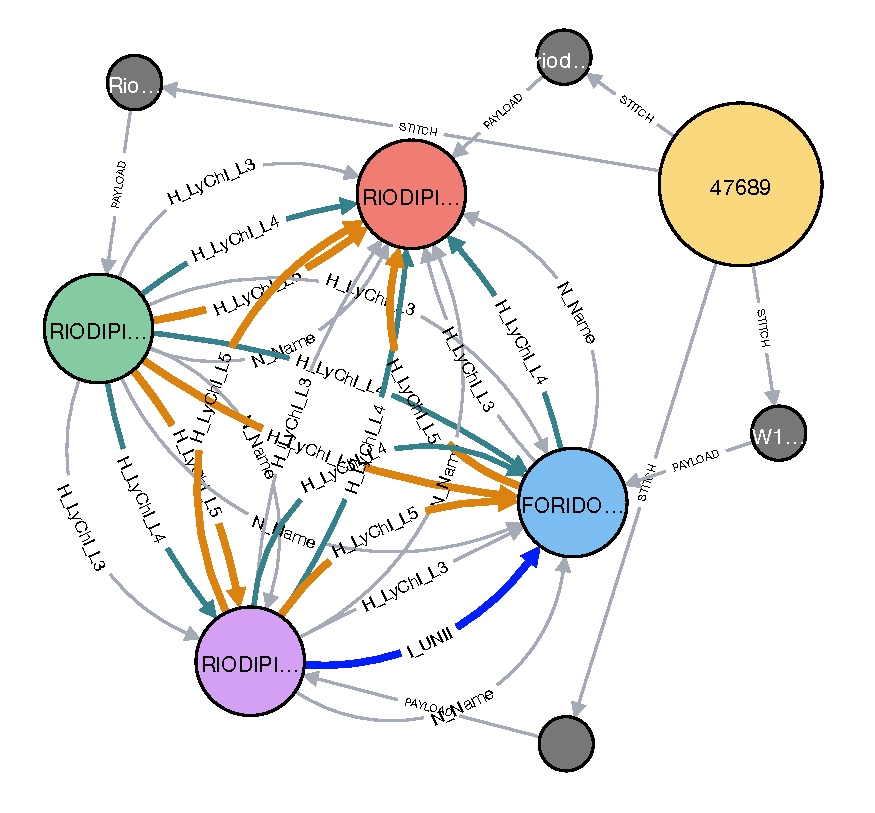
\includegraphics[scale=0.5]{graph3}}
\caption{A connected component in the stitch multigraph with four \emph{stitch nodes} (medium) and corresponding \emph{data nodes} (small). Each stitch value forms a clique within this connected component. The edge labels between stitch nodes are the stitch keys. The large node is the derived entity (i.e., sgroup node) generated from entity resolution.}\label{fig:graph1}
\end{figure}

\subsection{Stitch keys}
Stitch key is a core concept in \st. It defines how entities are matched, which, in turn, determines how cliques and connected components are formed. By virtue of its importance, the stitch key should reflect the true identity of the entity as much as possible. Depending on the entity type, the stitch key can be generic (e.g., synonym) or very specific (e.g., molecular hash key). For drug entity type, \st\ relies on the following stitch keys for each entity:
\begin{unlist}
\item{\texttt{N\_Name}.} This is the most generic stitch key available. Stitch values associated with this stitch key can be any established names or nomenclature; e.g., tradenames, INN (International Nonproprietary Names), USAN (United States Adopted Names), IUPAC (International Union of Pure and Applied Chemistry).
\item{\texttt{I\_UNII}, \texttt{I\_CAS}, \texttt{I\_CODE}.} These stitch keys represent (i) unique identifiers assigned to the entity by a well-known registrar (e.g., the U.S. Food and Drug Administration in the case of UNII) or (ii) internal company code. Both \texttt{I\_UNII} and \texttt{I\_CAS} are specific to drug (or substance in general) entity type, whereas \texttt{I\_CODE} can be used for any type of identifiers. The decision to use specific stitch keys over generic ones ultimately rests on the strategies used within entity resolution.
\item{\texttt{H\_LyChI\_L5}, \texttt{H\_LyChI\_L4}, \texttt{H\_LyChI\_L3}.} For the small molecule class of drugs, perhaps more important than any identifiers is the underlying chemical structure definition. These stitch keys are hash values derived from the molecular structure at different resolutions \citep{lychi}. Section~\ref{sec:methods-ingest} discusses in detail how these derived stitch values are generated.
\item{\texttt{R\_activeMoiety}.} Technically not a stitch key, the active moiety relationship between two drugs provides a strong evidence of equivalence. While this relationship can be infered directly from the chemical structures (e.g., freebase and salt forms, with and without esters), there is some level of curation needed to handle structures with metal complex.
\end{unlist}
Table~\ref{tab:imatinib} shows an example of stitch keys and stitch values for
the drug entity \emph{imatinib mesylate}. In this example, the \texttt{R\_activeMoiety} relationship specifies the UNII of the freebase form of imatinib mesylate.

\begin{table}[thb]
\processtable{Stitch keys and stitch values for the
drug \emph{imatinib mesylate}\label{tab:imatinib}}
{\begin{tabular}{@{}ll@{}}\toprule Stitch key &
Stitch value\\\midrule
\texttt{N\_Name} & \texttt{IMATINIB MESYLATE}; \texttt{GLEEVEC}; \texttt{GLIVEC}\\
\texttt{I\_UNII} & \texttt{8A1O1M485B}\\
\texttt{I\_CAS} & \texttt{220127-57-1}\\
\texttt{I\_CODE} & \texttt{STI-571}; \texttt{CHEMBL941}\\
\texttt{H\_LYCHI\_L5} & \texttt{7S4GKGNQ6N3X-N}\\
\texttt{H\_LYCHI\_L4} & \texttt{VLU17BQBSGWU-N}; \texttt{K83X3L3XSSHK-S}\\
\texttt{H\_LYCHI\_L3} & \texttt{VL3FPUQ59CU-N}; \texttt{K846NBMB7T3-S}\\
\texttt{R\_activeMoiety} & \texttt{BKJ8M8G5HI}\\\botrule
\end{tabular}}{}
\end{table}

\subsection{Data sources}
\st\ utilizes a number of diverse data sources for the \ix{} resource. Among the data sources, of particular importance is the public G-SRS data source from the FDA \citep{GSRSData}. This data source is well-curated and contains over 100K substances across six different classes: chemical, structurally diverse, protein, mixture, polymer, and nucleic acid. As a data source derived from the FDA's internal substance registry system, the G-SRS data source naturally forms the basis of our data integration effort. The complete list of data sources currently used by \st\ is shown in Table~\ref{tab:data-sources}.

\begin{table}[thb]
\processtable{\label{tab:data-sources}}
{\begin{tabular}{@{}ll@{}}\toprule
Data source & Size\\ \midrule
G-SRS, April 2019&	105,019\\
Withdrawn and Shortage Drugs List Feb 2018 &	674\\
Broad Institute Drug List 2018-09-07 &	6,125\\
NCATS Pharmaceutical Collection, April 2012 &	14,814\\
Rancho BioSciences, March 2019 &	51,591\\
Pharmaceutical Manufacturing Encyclopedia (Third Edition) &	2,268\\
DailyMed Rx, January 2019 &	74,850\\
DrugBank, December 2018&	11,922\\
DailyMed Other, January 2019&	13,393\\
DailyMed OTC, January 2019&	79,448\\
Drugs\@FDA \& Orange Book, July 2019&	28,256\\
ClinicalTrials, December 2017&	305,833\\
OTC Monographs, December 2018&	2,713\\
FDA NADA and ANADAs, December 2018&	554\\
FDA Excipients, December 2018&	10,212\\ \botrule
\end{tabular}}{}
\end{table}


\subsection{Overall strategy}
The basic premise behind \st{} is that data integration is often done within the context of a specific data source. This is a reasonable assumption given the data quality varies when integrating across disparate sources. Futhermore, by establishing a reference data source for data integration, we have finer control over the following:
\begin{unlist}
\item{\emph{Data quality}.} A reference data source is typically selected such that it is of high quality. Here, we can also impose other data quality constraints (e.g., no synonyms can span multiple entities) to guide entity resolution.
\item{\emph{Data resolution}.} Entity resolution is particularly challenging when data integration involves ontologies. A reference data source can serve as the anchor ontology from which other ontologies can be mapped. As with data quality, we can also impose any additional semantic constraints; e.g., prostate cancer is not one of the diagnoses for a female patient in an electronic health record.
\item{\emph{Data curation}.} Generating ground-truth data is more managable with a single data source than across multiple data sources. This is particularly important due to the iterative feedback between data curation and data integration.
\end{unlist}
The G-SRS data source serves as an ideal reference data source. Its rigorous substance models and well-structured data elements give us a good starting point for drug data integration. In the next section, we discuss our strategies in utilizing the G-SRS reference data source to address entity resolution for drug data.

\begin{methods}
\section{Methods}\label{sec:methods}
In general, data integration with \st{} consists of four basic steps: \emph{ingestion}, \emph{stitching}, \emph{entity resolution}, and \emph{entity normalization}. With the exception of \emph{entity resolution}, all other steps---as they are currently implemented in \st---are generic and can be applied to a wide range of entity types.

\subsection{Data ingestion}\label{sec:methods-ingest}
\st{} is capable of ingesting data in a wide variety of sources and formats. Semantic formats such as OWL, RDF, and Turtle are supported as are JSON, delimiter separated text, and custom formats. For non-semantic format, a separate configuration file is required to map properties to stitch keys.

An important step in data ingestion is the standaridzation and validation of stitch values. For \texttt{N\_Name} stitch key, the standardization procedure is simply to convert the input string to uppercase; no validation is performed. For \texttt{I\_UNII} and \texttt{I\_CAS} stitch keys, no standardization is required, and validation is a simple checksum calculation to ensure the stitch value is proper. Depending on the input format, \st\ also provides basic utilities (e.g., regular expression) to help with data transformation during ingestion.

Perhaps the most unique feature of \st\ is its ability to incorporate knowledge of chemical structures into entity resolution. Whereas traditional approaches rely on names and identifiers to determine equivalence relation among substances, \st\ goes a step further and utilizes the underlying chemical structures to infer equivalence. This is particularly relevant when the drug is a mixture, prodrug, or active moiety with complex excipient (or derivative thereof). As an example, consider the drug entity \emph{IMATINIB MESYLATE} and its active ingredient \emph{IMATINIB}. Here, it is obvious that the two entities cannot be matched by name alone. Instead, having structural information by way of molecular hash keys for each molecular component allows us to determine equivalence from the common active moiety \emph{IMATINIB} between the two entities. This trivial example might suggest that, instead of comparing names exactly, we find the longest common substring of the names. The approach would certainly work in this example, but to make it work in general would require very specialized parsing rules and dictionaries.

For data sources with chemical structures, the most computationally demanding step in data ingestion is the generation of molecular hash keys. Hash keys are generated for each component of a chemical structure in three different structural levels: \texttt{L5}, \texttt{L4}, and \texttt{L3}, which correspond to stitch keys \texttt{H\_LYCHI\_L5}, \texttt{H\_LYCHI\_L4}, and \texttt{H\_LYCHI\_L3}, respectively. Level \texttt{L5} is the most specific; it represents the chemical structure as-is, i.e., without structure normalization and standardization. With the exception of the relation \texttt{R\_activeMoiety}, a match at this level has higher priority over other stitch keys. The next level \texttt{L4} represents the structure after normalization and standardization per the LyChI software package \citep{lychi}. A match at this level implies that two structures are equivalent
%insofar as \textcolor{red}{the valence bond theory is valid}
in terms of stereochemistry, resonance, and tautomerism. And the last level \texttt{L3} is the same as \texttt{L4} but without stereochemistry. A match at this level is considered weak and does not constitute equivalence without other significant supporting evidence. The purpose for \texttt{L3} is in anticipation of incorrect or missing stereo information, which is one of the most common type of errors associated with chemical structures. For each hash key, a suffix \texttt{-M}, \texttt{-S}, or \texttt{-N} is also assigned to designate the molecular component as either a \emph{metal}, \emph{salt}, or \emph{neither}, respectively. Table~\ref{tab:imatinib} illustrates all three representations for the drug \emph{IMATINIB MESYLATE}. Note that the cardinality for \texttt{L5} is always one, whereas for \texttt{L4} and \texttt{L3} the cardinality is equal to the number of non-hydrate molecular components. (Hydrate components are removed prior to processing.)

\subsection{Data stitching}
\emph{Stitching} is the process by which the stitch multigraph is incrementally constructed as data is ingested. Algorithm~\ref{algo:stitching} describes the basic stitching algorithm in \st. This algorithm is applied to each data source, and upon its completion yields a stitch multigraph such that any stitch value that spans $N$ stitch nodes forms an induced clique, i.e., a complete subgraph of $N$ nodes and $\frac{N(N-1)}{2}$ edges. Overlapping induced cliques form the basis for the proposed entity resolution approach discussed in the next section.

\begin{algorithm}\label{algo:stitching}
\SetKwInOut{Input}{Input}
\SetKwInOut{Output}{Output}
\SetKwFunction{Union}{Union}
\SetKwFunction{Find}{Find}
\SetAlgoLined
\DontPrintSemicolon
Let $W$ denote the set of stitch nodes created in the data ingestion step for a given data source $D$.\\
Let $\langle k, v\rangle$ be the tuple of stitch key and value, respectively, defined for a stitch node $w$.\\
$G=(V,E)$ is current stitch multigraph.\\
\Find{$k, v$} is a function that returns all stitch nodes in $V$ containing stitch key $k$ and stitch value $v$.\\
\Union{$w,z$} is a union-find algorithm for tracking disjoint sets (i.e., connected components).\\
 \For{$w \in W$}{
    \For{$\langle k_i, v_i\rangle \in w$}{
      \For{$z \in$ \Find{$k_i,v_i$}}{
         $E \leftarrow E \cup z\thicksim w$\;
         \Union{$w,z$}\;
      }
    }
    $V \leftarrow V \cup w$\;
 }
 \caption{Entity stitching algorithm}
\end{algorithm}

\subsection{Entity resolution}\label{sec:methods-er}

\subsection{Entity normalization}

%\enlargethispage{6pt}
\end{methods}

\section{Results}

%\begin{figure}[!tpb]%figure2
%%\centerline{\includegraphics{fig02.eps}}
%\caption{Caption, caption.}\label{fig:02}
%\end{figure}


\section{Discussion}


%%%%%%%%%%%%%%%%%%%%%%%%%%%%%%%%%%%%%%%%%%%%%%%%%%%%%%%%%%%%%%%%%%%%%%%%%%%%%%%%%%%%%
%
%     please remove the " % " symbol from %\centerline{\includegraphics{fig01.eps}}
%     as it may ignore the figures.
%
%%%%%%%%%%%%%%%%%%%%%%%%%%%%%%%%%%%%%%%%%%%%%%%%%%%%%%%%%%%%%%%%%%%%%%%%%%%%%%%%%%%%%%

\section*{Acknowledgements}

We thank our colleagues, Mark Williams and Tyler Beck, for their valuable proof-reading of early drafts of the manuscript. We also thank our colleague, Tongan Zhao, for his help in developing a prototype curation user interface for \st.

\bibliographystyle{natbib}
%\bibliographystyle{achemnat}
%\bibliographystyle{plainnat}
%\bibliographystyle{abbrv}
%\bibliographystyle{bioinformatics}
%
%\bibliographystyle{plain}
%
\bibliography{stitcher}
\end{document}
